This monograph is part of the longstanding project of exploring connections between logic and combinatorics. Our focus is, more specifically, on studying the computable (or effective) content of combinatorial theorems. This has a long history, as we survey below. The interest stems from the realization that combinatorial notions tend to be computability-theoretically natural, and vice-versa. Traditionally, this has led to fine-grained analyses of different combinatorial constructions, often resulting in new, more computationally efficient proofs of various combinatorial results.

Over time, this work has made increasing use of powerful set-theoretic and combinatorial techniques, whose adaptation to the realm of computability theory has produced new insights into unsolved problems. Such will be the case for our investigation here of Milliken's tree theorem (named for its author, and originally proved in~\cite{Milliken1979RTforTrees}; cf. also~\cite{Milliken1881}). This is a deep result whose significance in Ramsey theory and related areas has made it the objective of much attention in combinatorics and set theory. This makes all the more surprising its near complete absence from the computability-theoretic literature. To our knowledge, the only published mentions are by Carlson and Simpson \cite[Section 3]{Carlson1984dual} and Chubb, Hirst, and McNicholl~\cite{Chubb2009Reverse}. The authors of the former paper introduce the so-called dual Ramsey's theorem, and give as a consequence a new proof of the Halpern-La\"{u}chli theorem, an important result for understanding Milliken's tree theorem that we investigate at length also here. The latter paper focuses on what is ultimately a kind of weak or degenerate form of Milliken's tree theorem, which has garnered a great deal of interest in its own right. See \Cref{sec:GenCHMTT}, where we give a full account of the theorem of Chubb, Hirst, and McNicholl and how it relates to Milliken's in the context of our work here. (We add that during the writing of this manuscript, we learned of a concurrent project of Chong, Li, Liu, and Yang in progress, whose focus is the Chubb, Hirst, and McNicholl theorem but which also obtains results about Milliken's tree theorem proper. Specifically, the authors obtain by independent means our \Cref{thm:milliken-aca} below.)

The problem of determining the computable content of Milliken's tree theorem was proposed by Dobrinen~\cite{Dobrinen-2018}. We give a complete analysis here, using the tools of computability theory and reverse mathematics. As we will show, Milliken's tree theorem turns out to be surprisingly rich and intricate in this respect, reflecting its centrality among other partition theorems, including Ramsey's theorem and its many variants.

\section{Milliken's tree theorem and Ramsey theory}

Ramsey theory is a vast area of combinatorics, broadly interested in results about when some sort of regularity is unavoidable when a large given structure is partitioned into a small number of pieces. (Here ``large'' is typically taken to mean a particular finite or infinite cardinality, and ``small'' is understood relative to this cardinality.) Canonical examples include, of course, the finite and infinite Ramsey's theorems, both due to F.~P.~Ramsey~\cite{Ramsey1929}, which we recall. Let $\NN$ denote the set of natural numbers, $\{0,1,2,\ldots\}$, and given a set $X \subseteq \NN$ and integer $n \geq 1$, let $[X]^n = \{ ( x_0,\ldots,x_{n-1} ) \in X^n: x_0 < \cdots < x_{n-1}\}$. We identify each $k \in \NN$ with the set of its predecessors, $\{0,1,\ldots,k-1\}$.
%Given a function $f$ defined on a set $X$ let $f \upharpoonright Y$ denote its restriction to $Y \subseteq X$.

\index{Ramsey's theorem!finite}
\begin{theorem}[Finite Ramsey's theorem]
	For all $n,k, \geq 1$ and $m_1$,$\ldots$, $m_{k-1} \in \NN$ there is a number $M \in \NN$ such that for every $f: [M]^n \to k$ there is an $i < k$ and a set $H \subseteq M$ of size $m_i$ such that $f(\vec{x}) = i$ for all $\vec{x} \in [H]^n$.
\end{theorem}

\index{Ramsey's theorem!infinite}
\begin{theorem}[Infinite Ramsey's theorem]
	For all $n,k \geq 1$ and every $f: [\NN]^n \to k$ there is an $i < k$ and an infinite set $H \subseteq \NN$ such that $f(\vec{x}) = i$ for all $\vec{x} \in [X]^n$.
\end{theorem}

\index{homogeneous set!for a coloring}
\noindent The sets $H$ above are called \emph{homogeneous sets} for the coloring $f$. There are also versions of Ramsey's theorem for colorings of uncountable sets, but we will restrict our attention here to the countable setting.

In broad strokes, Ramsey's theorem(s) can be seen as saying that in any configuration of integers, however complicated or random, some amount of order is necessary. Understanding this order, and how it arises, is naturally captivating, and its study has resulted in important advances across mathematics, from combinatorics to logic to number theory. These include, for example, the celebrated Szemer\'{e}di's theorem (cf.~\cite{Szemeredi1975,Szemeredi1975b}), the various proofs of which over the years, and the myriad mathematical ideas used in them, led to it be called the ``Rosetta stone'' of mathematics by Tao~\cite{Tao2007}. We will explore a number of other examples in this monograph. For a general introduction to Ramsey theory, we refer the reader to the book of Graham, Rothschild, and Spencer~\cite{GRS2013}. For more background on the kind of combinatorics most relevant to us here, we refer to Todorcevic~\cite{Todorcevic2010Ramsey}.

The main subject of the present monograph, Milliken's tree theorem, is a strong generalization of the infinite Ramsey's theorem. We state it here in a restricted form in order to be able to begin discussing it. The full statement requires more nuanced definitions that we delay until the next chapter. For now, we recall that $2^{<\omega}$ denotes the set of all finite binary strings, i.e., finite sequences of $0$s and $1$s. For $\sigma \in 2^{<\omega}$, we write $|\sigma|$ for the length of $\sigma$, i.e., the number of bits occurring in $\sigma$, and we let $2^n$ and $2^{<n}$ denote the sets of $\sigma \in 2^{<\omega}$ with $|\sigma| = n$ and $|\sigma| < n$, respectively. For $\sigma,\tau \in 2^{<\omega}$ we write $\sigma \preceq \tau$ to mean that $\sigma$ is an initial segment (not necessarily proper) of $\tau$, and $\sigma \prec \tau$ to mean $\sigma \preceq \tau$ and $\sigma \neq \tau$. We also write $\sigma \meet \tau$ for the longest common initial segment of $\sigma$ and $\tau$. The crucial notion in the statement of Milliken's tree theorem is the following: $S \subseteq 2^{<\omega}$ is a \emph{strong subtree of $2^{<\omega}$} if $S$ is closed under $\meet$, and $(S,\preceq)$ is isomorphic, as a structure, to either $(2^{<\omega},\preceq)$ or $(2^{< n},\preceq)$ for some $n$, via a map that preserves whether or not a pair of nodes has the same length. Thus, for instance, $\{ \str{01}, \str{0101}, \str{0110} \}$ is a strong subtree of $2^{<\omega}$, whereas $\{ \str{01}, \str{0100}, \str{0101} \}$ and $\{ \str{01}, \str{0101}, \str{011} \}$ are not, even though all three sets, under $\preceq$, are isomorphic to $(2^{< n},\preceq)$. (See \Cref{f:intro}.)

\begin{figure}[h]
\centering
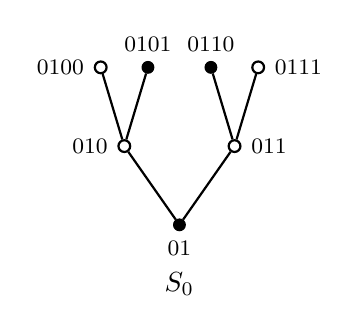
\begin{tikzpicture}[font=\footnotesize]
	\tikzset{
		empty node/.style={circle,inner sep=0,fill=none},
		solid node/.style={circle,draw,inner sep=1.5,fill=black},
		hollow node/.style={circle,draw,inner sep=1.5,thick}
	}
	\tikzset{snake it/.style={decorate, decoration=snake, line cap=round}}
	\node(01)[solid node,label=below:{$01$}] at (0,0) {};
	\node(010)[hollow node,label=left:{$010$}] at (-0.7,1) {};
	\node(011)[hollow node,label=right:{$011$}] at (0.7,1) {};
	\node(0100)[hollow node,label=left:{$0100$}] at (-1,2) {};
	\node(0101)[solid node,label=above:{$0101$}] at (-0.4,2) {};
	\node(0110)[solid node,label=above:{$0110$}] at (0.4,2) {};
	\node(0111)[hollow node,label=right:{$0111$}] at (1,2) {};
	\draw[-,thick] (01) to (010);
	\draw[-,thick] (01) to (011);
	\draw[-,thick] (010) to (0100);
	\draw[-,thick] (010) to (0101);
	\draw[-,thick] (011) to (0110);
	\draw[-,thick] (011) to (0111);
	\node at (0,-0.75) {\normalsize $S_0$};
\end{tikzpicture}
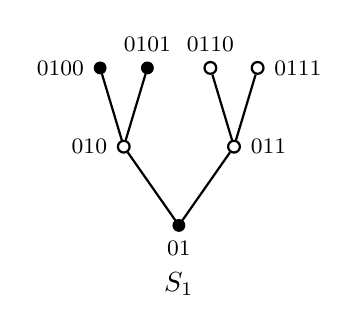
\begin{tikzpicture}[font=\footnotesize]
	\tikzset{
		empty node/.style={circle,inner sep=0,fill=none},
		solid node/.style={circle,draw,inner sep=1.5,fill=black},
		hollow node/.style={circle,draw,inner sep=1.5,thick}
	}
	\tikzset{snake it/.style={decorate, decoration=snake, line cap=round}}
	\node(01)[solid node,label=below:{$01$}] at (0,0) {};
	\node(010)[hollow node,label=left:{$010$}] at (-0.7,1) {};
	\node(011)[hollow node,label=right:{$011$}] at (0.7,1) {};
	\node(0100)[solid node,label=left:{$0100$}] at (-1,2) {};
	\node(0101)[solid node,label=above:{$0101$}] at (-0.4,2) {};
	\node(0110)[hollow node,label=above:{$0110$}] at (0.4,2) {};
	\node(0111)[hollow node,label=right:{$0111$}] at (1,2) {};
	\draw[-,thick] (01) to (010);
	\draw[-,thick] (01) to (011);
	\draw[-,thick] (010) to (0100);
	\draw[-,thick] (010) to (0101);
	\draw[-,thick] (011) to (0110);
	\draw[-,thick] (011) to (0111);
	\node at (0,-0.75) {\normalsize  $S_1$};
\end{tikzpicture}
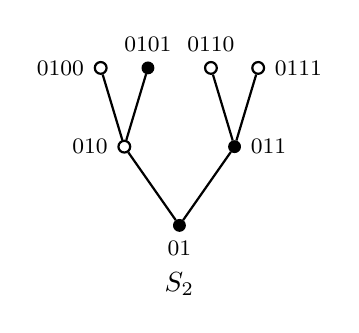
\begin{tikzpicture}[font=\footnotesize]
	\tikzset{
		empty node/.style={circle,inner sep=0,fill=none},
		solid node/.style={circle,draw,inner sep=1.5,fill=black},
		hollow node/.style={circle,draw,inner sep=1.5,thick}
	}
	\tikzset{snake it/.style={decorate, decoration=snake, line cap=round}}
	\node(01)[solid node,label=below:{$01$}] at (0,0) {};
	\node(010)[hollow node,label=left:{$010$}] at (-0.7,1) {};
	\node(011)[solid node,label=right:{$011$}] at (0.7,1) {};
	\node(0100)[hollow node,label=left:{$0100$}] at (-1,2) {};
	\node(0101)[solid node,label=above:{$0101$}] at (-0.4,2) {};
	\node(0110)[hollow node,label=above:{$0110$}] at (0.4,2) {};
	\node(0111)[hollow node,label=right:{$0111$}] at (1,2) {};
	\draw[-,thick] (01) to (010);
	\draw[-,thick] (01) to (011);
	\draw[-,thick] (010) to (0100);
	\draw[-,thick] (010) to (0101);
	\draw[-,thick] (011) to (0110);
	\draw[-,thick] (011) to (0111);
	\node at (0,-0.75) {\normalsize $S_2$};
\end{tikzpicture}
\caption{Three subsets, $S_0$, $S_1$, and $S_2$, of $2^{<\omega}$. Solid circles indicate strings in the set, hollow circles strings not in the set. Only $S_0$ is a strong subtree of $2^{<\omega}$.}\label{f:intro}
\end{figure}

Given $T \subseteq 2^{<\omega}$, let $\mathcal{S}_\omega(T)$ denote the set of strong subtrees of $2^{<\omega}$ that are contained in $T$ and isomorphic to $(2^{<\omega},\preceq)$. For $n \geq 1$, let $\mathcal{S}_n(T)$ denote the set of strong subtrees of $2^{<\omega}$ that are contained in $T$ and isomorphic to $(2^{< n},\preceq)$.

\index{Milliken's tree theorem!for $2^{<\omega}$}
\index{tree theorem!Milliken's tree theorem}
\index{theorem!Milliken's tree theorem}
\begin{theorem}[Milliken's tree theorem for $2^{<\omega}$]
	For all $n,k \geq 1$ and all $f: \mathcal{S}_n(2^{<\omega}) \to k$ there exists $i < k$ and a $T \in \mathcal{S}_\omega(2^{<\omega})$ such that $f(S) = i$ for all $S \in \mathcal{S}_n(T)$.
\end{theorem}

To begin, note that the infinite Ramsey's theorem is a straightforward consequence of (even this version of) Milliken's tree theorem. Indeed, given a coloring $f: [\NN]^n \to k$, we define $g: \mathcal{S}_n(2^{<\omega}) \to k$ as follows. For each $S \in \mathcal{S}_n(2^{<\omega})$, let $\vec{x}_S = \{ |\sigma|: \sigma \in S\}$, which is a set of size $n$ and so can be viewed as an element of $[\NN]^n$. Let $g(S) = f(\vec{x}_S)$. Now if $T \in \mathcal{S}_\omega(2^{<\omega})$ is as given by Milliken's tree theorem for this $g$, then $H = \{|\sigma|: \sigma \in T\}$ is easily seen to be an infinite homogeneous set for $f$.

Indeed, it is well-known that Milliken's tree theorem implies a great many partition theorems, including a number that are significantly more difficult to prove than Ramsey's. We will look at several of these theorems in this manuscript, and show that their implications from Milliken's tree theorem can be made constructive in the sense of computability theory and reverse mathematics, which we discuss below. Much of this will rely on carefully identifying and examining features common between strong subtrees of $2^{<\omega}$ and the combinatorial structures underlying these other principles, using a combination of ideas that have previously been successfully employed in structural Ramsey theory, along with techniques newly developed here.

We refer the reader to Todorcevic~\cite[Chapter 6]{Todorcevic2010Ramsey} for an in-depth discussion of Milliken's tree theorem, and a careful development of a proof. As with Ramsey's theorem, the proof has an inductive form based on the exponent, $n$, of the colorings being considered. Thus, we prove it first for finite colorings of $\mathcal{S}_1(2^{<\omega})$, and then assuming it holds for finite colorings of $\mathcal{S}_n(2^{<\omega})$, we prove it for finite colorings of $\mathcal{S}_{n+1}(2^{<\omega})$. The base case, $n = 1$, is actually not difficult to prove directly (though it is less trivial than the $n = 1$ case of Ramsey's theorem, i.e., the infinitary pigeonhole principle). However, unlike in standard proofs of Ramsey's theorem, where the inductive step uses just the $n = 1$ case to increase the exponent, in the case of Milliken's tree theorem a stronger result is needed. This is the so-called Halpern-La\"{u}chli theorem, due originally to Halpern and La\"{u}chli \cite{HalperbLauchli1966}, and independently Laver (unpublished) and Pincus \cite{Pincus1974} (see \cite{Pincus1981} for more on the history).

Given $d \geq 1$ and $T_0,\ldots,T_{d-1} \subseteq 2^{<\omega}$, let $\mathcal{S}_\alpha(T_0,\ldots,T_{d-1})$ for $\alpha \in \NN \cup \{\omega\}$ be the collection of all tuples $(S_0,\ldots,S_{d-1})$ such that for each $i < d$ we have $S_i \in \mathcal{S}_\alpha(T_i)$, and for all $i,j < d$ and all $\sigma \in S_i$ and $\tau \in S_j$, we have that $\sigma$ has the same number of initial segments in $S_i$ as $\tau$ does in $S_j$ if and only if $|\sigma| = |\tau|$.

\index{Halpern-La\"{u}chli theorem!for $2^{<\omega}$}
\index{theorem!Halpern-La\"{u}chli theorem}
\begin{theorem}[Halpern-La\"{u}chli theorem for $2^{<\omega}$]
	For all $d,k \geq 1$ and all $f: \bigcup_{n \in \NN} (2^n)^d \to k$ there exists $i < k$ and $(T_0,\ldots,T_{d-1}) \in \mathcal{S}_\omega(2^{<\omega},\ldots,2^{<\omega})$ such that $f(\vec{\sigma})=i$ for all $\vec{\sigma} = (\sigma_0,\ldots,\sigma_{d-1}) \in T_0 \times \cdots \times T_{d-1}$ with $|\sigma_0| = \cdots = |\sigma_{d-1}|$.
\end{theorem}

\noindent Prima facie, this theorem appears as a kind of parallelized version of Milliken's tree theorem for colorings of $\mathcal{S}_1(2^{<\omega})$, and one may expect it to be not much more complicated to prove. In fact, this is misleading, and the Halpern-La\"{u}chli theorem largely encompasses the entire combinatorial core of (the full) Milliken's tree theorem. We will analyze the Halpern-La\"{u}chli theorem in detail in this monograph, and use it in a careful way to give a more effective proof of Milliken's tree theorem.

\section{Computable combinatorics}

\index{$\leq_T$}
\index{$\equiv_T$}
\index{computable}
\index{Turing!reduction}
\index{halting problem}
\index{Turing!equivalence}
The principal theme of modern computability theory is \emph{relative} computability: a set $X \subseteq \NN$ is \emph{computable from} (or \emph{Turing reducible to}) a set $Y$, written $X \Tred Y$, if there is an algorithm to decide which numbers belong to $X$ using information about which numbers belong to $Y$. If $X \Tred Y$ and $Y \Tred X$ we write $X \Tequiv Y$. This notion, along with a precise formalization of the concept of an algorithm, was a seminal achievement of Turing in the 1930s. Sets can be classified in numerous ways, such as in terms of their structural properties or by their syntactic descriptions.

As a rule, all such properties can be \emph{relativized}, leading to increasingly larger classes of sets. For example, the \emph{halting problem relative to $X$}, denoted $X'$ and also called the \emph{(Turing) jump of $X$}, refers to the set of $e \in \NN$ such that the $e$th algorithm in some fixed listing, with access to information about $X$, halts on input $e$. For every $X$ we have that $X \Tred X'$ but $X' \nTred X$, which yields in particular a canonical example of a non-computable set. The complexity of a set of natural numbers in computability theory (or by extension, of any object that can be naturally represented or encoded by such a set) is a measure of ``how far'' it is from being computable, according to various hierarchies of classes of sets obtained in this fashion. For general background in computability theory, we refer the reader to Soare~\cite{Soare2016Turing} and to Downey and Hirschfeldt~\cite{Downey2010Algorithmic}.

Computability theory lends itself to analyzing a vast collection of problems that are sometimes called \emph{instance-solution problems}\index{problem}. This refers to theorems having the form
\begin{equation}\label{eqn:Pi12}
	\forall A~[\mathrm{P}(A) \implies \exists B~\mathrm{Q}(A,B)],
\end{equation}
where $\mathrm{P}$ and $\mathrm{Q}$ are some sort of properties of $A$, and of $A$ and $B$, respectively. One can regard such a theorem as the problem, ``Given an $A$ such that $\mathrm{P}(A)$ holds, find a $B$ such that $\mathrm{Q}(A,B)$ holds''. In this context, we call such $A$ the \emph{instances} of the problem (or theorem), and all such $B$ the \emph{solutions} to $A$. This is a natural way of thinking about theorems of this shape. For example, the instances of Ramsey's theorem are all finite colorings of $[\omega]^n$ for some $n$, and the solutions to any such coloring are its infinite homogeneous sets.

One way to gauge the complexity of an instance-solution problem is by studying the relationship between the complexity of instances and solutions, when these can be presented as subsets of $\NN$, as will be the case in all the examples we consider in this manuscript. From this perspective, a problem that is \emph{computably true}\index{computably true}, i.e., one each of whose instances has at least one solution computable in that instance, is trivial from the algorithmic standpoint. By contrast, a problem that has an instance all of whose solutions compute the jump of that instance, is strictly harder, being, in a certain sense, at least as difficult as ``solving the halting problem''. In general, the further apart the instances and solutions are in this sense, the more algorithmically complex it is. We can thus directly compare different problems in terms of their complexity, yielding a notion of algorithmic or computability-theoretic strength. For a thorough introduction to this kind of analysis, which is generally called \emph{computable mathematics}, see the book of Hirschfeldt~\cite{Hirschfeldt2015Slicing}.


A complementary approach is provided by the foundational program of \emph{reverse mathematics}\index{reverse mathematics}, developed by Friedman and Simpson in the late 1970s. The setting here is second-order arithmetic, a formal system strong enough to express countable analogues of most results of classical mathematics. Its axioms include the usual ordered semi-ring axioms for the natural numbers, together with \emph{comprehension axioms} asserting that the set of all numbers $x$ satisfying a given formula (property) exists. By restricting to only certain kinds of formulas we get various \emph{subsystems} of second-order arithmetic, the most basic of which is called $\RCA_0$ and roughly corresponds to computable mathematics. The traditional approach in the subject has been to compare a given theorem with several benchmark subsystems ($\WKL_0$, $\ACA_0$, $\ATR_0$) extending $\RCA_0$, corresponding to increasing levels of non-constructibility. Isolating the weakest such system that the theorem can be proved in, and the strongest that can in turn be proved from it over the base system $\RCA_0$, yields a measure of its proof-theoretic strength. There is a fruitful and well-understood interplay between reverse mathematics and computability theory, with ideas and results from one often leading to results in the other (see Shore~\cite{Shore1975Splitting}). This has been made even more pronounced in recent years by the introduction of various Weihrauch-style reducibilities to the subject, which have come to be viewed largely as an extension and refinement of the traditional program of reverse mathematics. Computable reducibility\index{computable!reducibility}, in particular, which is a non-uniform analogue of Weihrauch reducibility originally introduced in~\cite{Dzhafarov2014Cohesive}, will figure in a number of our results here.

The standard reference on reverse mathematics is Simpson~\cite{Simpson2009Subsystems}. Weihrauch reducibility was introduced by Weihrauch \cite{Weihrauch1992} in the 1990s, and has since been widely deployed in computable analysis and other fields; for a recent survey, see Brattka, Gherardi, and Pauly~\cite{BrattkaSurvey}.

Of course, instance-solution problems are ubiquitous across mathematics, but problems from combinatorics have figured especially prominently in the above frameworks for many decades. The classification and differentiation of combinatorial theorems according to their computability-theoretic and proof-theoretic strength is nowadays called \emph{computable combinatorics}. Perhaps the earliest result here is the following one from the late 1960s, stating that Ramsey's theorem for pairs is not computably true.

\begin{theorem}[Specker~\cite{Specker-1971}]
	There is a computable $f: [\omega]^2 \to 2$ with no computable infinite homogeneous set.
\end{theorem}
 
\noindent (In the parlance of reverse mathematics, this shows that Ramsey's theorem for colorings of pairs is not provable in the base theory, $\RCA_0$.) This result was greatly extended in the seminal 1972 paper of Jockusch~\cite{Jockusch1972Ramseys}, which set off an industry of research on Ramsey's theorem in computability theory that is still highly active today.
 
The computability-theoretic perspective offers insights that are not readily discernible in combinatorics alone. In the case of Ramsey's theorem, a well-known example is provided by the following pair of results.

\begin{theorem}[Jockusch~\cite{Jockusch1972Ramseys}, Theorem 5.7]
	For each $n \geq 3$, there is a computable $f: [\omega]^n \to 2$ each of whose infinite homogeneous sets computes $\emptyset^{(n-2)}$ (and in particular $\emptyset'$).
\end{theorem}
 
\begin{theorem}[Seetapun; see~\cite{Seetapun1995strength}]\label{thm:Seetapun}
	Every computable $f: [\omega]^2 \to 2$ has an infinite homogeneous set that does not compute $\emptyset'$.	
\end{theorem}
 
\noindent Thus, there is a direct computational distinction between Ramsey's theorem for colorings of pairs and Ramsey's theorem for colorings triples and larger tuples. (Formalizing these results in $\RCA_0$ yields that Ramsey's theorem for colorings of triples implies the system $\ACA_0$ over $\RCA_0$, whereas Ramsey's theorem for colorings of pairs does not.)

 
Such threshold phenomenon, where an increase in a parameter changes a theorem from not being able to encode specific non-computable information to being able to do so, are observed quite widely. For example, as was shown by Dzhafarov and Patey~\cite{Dzhafarov2017Coloring}, this is the case for the aforementioned theorem introduced by Chubb, Hirst, and McNicholl \cite{Chubb2009Reverse}. And more recently, Chong et al.~\cite{Chong2019Strengthc} obtained similar results for a theorem of Erd\H{o}s and Rado about colorings of pairs of rationals. We will likewise establish threshold phenomena for Milliken's tree theorem and the various consequences of it we consider.

Another computability-theoretic feature that will feature prominently in our work is \emph{cone avoidance}\index{cone avoidance}. In the subject, a \emph{cone} refers to a set of subsets of $\omega$ closed upward under $\Tred$. As a case in point, the set of all sets $X$ that compute $\emptyset'$ is a cone, and Seetapun's theorem (\Cref{thm:Seetapun} above) can be seen as saying that every computable instance of Ramsey's theorem for colorings of pairs has a solution that lies outside (or avoids) this cone. The emphasis here is on the restriction to \emph{computable instances}, however; indeed, it is easy to see that there is a (necessarily non-computable) $f: [\omega]^2 \to 2$, each of whose infinite homogeneous sets \emph{does} compute $\emptyset'$. By contrast, some instance-solution problems enjoy a stronger property called \emph{strong cone avoidance}\index{strong cone avoidance}\index{cone avoidance!strong}, whereby \emph{every} instance (computable or not) has at least one solution that avoids the cone of sets that compute $\emptyset'$. This is the case, for example, for the infinitary pigeonhole principle, as shown by Dzhafarov and Jockusch~\cite[Lemma 3.2]{Dzhafarov2009Ramseys}. We shall investigate both cone avoidance and strong cone avoidance for versions of Milliken's tree theorem, and in particular, for the Halpern-La\"{u}chli theorem. It is worth noting, too, that while every computably true problem obviously possesses cone avoidance, not every such problem satisfies strong cone avoidance. (For example, consider the identity problem, whose instances are all $X \subseteq \omega$, and the only solution of $X$ is $X$ itself.)
 
\section{Plan of the manuscript}

The manuscript is organized as follows. In \Cref{sec:defns}, we give further background and definitions to allow us to state the full versions of Milliken's tree theorem and the Halpern-La\"{u}chli theorem. In \Cref{sect:hl-theorem}, we proceed to the computability-theoretic analysis of the Halpern-Lauchli theorem, as a bootstrap to understanding the computational content of Milliken's tree theorem. In particular, we prove that the Halpern-Lauchli theorem is computably true (\Cref{thm:halpern-lauchli-computably-true}) and admits strong cone avoidance (\Cref{thm:hl-strong-cone-avoidance}). Then, in \Cref{sect:milliken-theorem}, we analyse a product version of Milliken's tree theorem. We prove that the statement is equivalent to $\ACA_0$ for strong subtrees of height at least $3$ (\Cref{thm:milliken-aca}), and that its restriction to colorings of strong subtrees of height 2 admits cone avoidance (\Cref{thm:cone-avoidance-MTT2}). Lastly, we prove that a weakening to the product version of Milliken's tree theorem for height 3, for which the solutions have now at most 2 colors instead of 1, admits cone avoidance (\Cref{thm:pmtt3k2-cone-avoidance}). In \Cref{sect:applications}, we study three applications of Milliken's tree theorem for pairs, namely: Devlin's theorem concerning colorings of tuples of rationals; a theorem about colorings of finite subgraphs of the Rado graph; and a generalization of the combinatorial theorem of Chubb, Hirst, and McNicholl discussed above. Finally, in \Cref{sect:open-questions}, we state some questions that our investigation leaves open.